\documentclass[tikz,border=8pt]{standalone}
\usepackage{amsmath}
\usetikzlibrary{arrows.meta,positioning,fit,calc}

\begin{document}
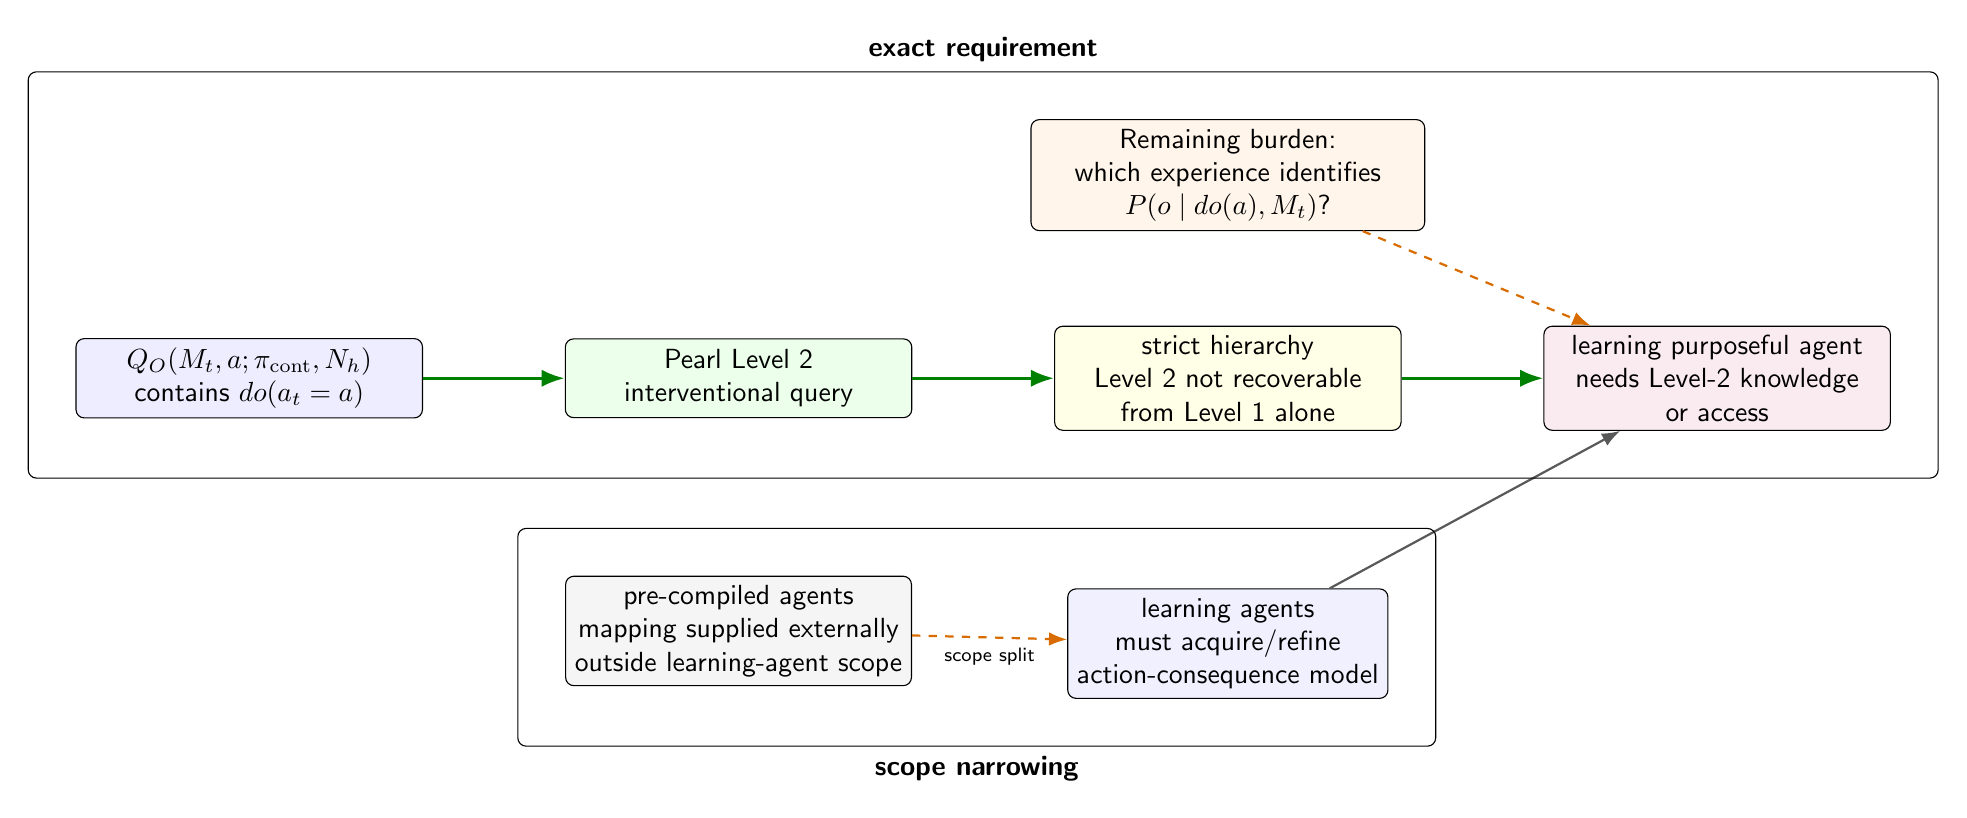
\begin{tikzpicture}[
  font=\sffamily,
  box/.style={draw, rounded corners=3pt, align=center, minimum width=36mm, minimum height=9mm, fill=white},
  wide/.style={draw, rounded corners=3pt, align=center, minimum width=44mm, minimum height=10mm, fill=white},
  arrow/.style={-Latex, thick, draw=black!65},
  good/.style={-Latex, very thick, draw=green!50!black},
  cut/.style={-Latex, thick, dashed, draw=orange!85!black},
  note/.style={align=center, font=\sffamily\scriptsize}
]

\node[wide, fill=blue!7] (q) {$Q_O(M_t,a;\pi_{\rm cont},N_h)$\\contains $do(a_t=a)$};
\node[wide, right=18mm of q, fill=green!8] (l2) {Pearl Level 2\\interventional query};
\node[wide, right=18mm of l2, fill=yellow!10] (noncollapse) {strict hierarchy\\Level 2 not recoverable\\from Level 1 alone};
\node[wide, right=18mm of noncollapse, fill=purple!8] (need) {learning purposeful agent\\needs Level-2 knowledge\\or access};

\draw[good] (q) -- (l2);
\draw[good] (l2) -- (noncollapse);
\draw[good] (noncollapse) -- (need);

\node[box, below=20mm of l2, fill=gray!8] (pre) {pre-compiled agents\\mapping supplied externally\\outside learning-agent scope};
\node[box, below=20mm of noncollapse, fill=blue!6] (learn) {learning agents\\must acquire/refine\\action-consequence model};
\draw[cut] (pre) -- node[below, note] {scope split} (learn);
\draw[arrow] (learn) -- (need);

\node[box, above=12mm of noncollapse, fill=orange!8, minimum width=50mm] (caveat)
  {Remaining burden:\\which experience identifies\\$P(o\mid do(a),M_t)$?};
\draw[cut] (caveat) -- (need);

\node[draw, rounded corners=3pt, fit=(q)(l2)(noncollapse)(need)(caveat), inner sep=6mm,
  label={[font=\sffamily\bfseries]above:exact requirement}] {};
\node[draw, rounded corners=3pt, fit=(pre)(learn), inner sep=6mm,
  label={[font=\sffamily\bfseries]below:scope narrowing}] {};

\end{tikzpicture}
\end{document}
